% ============================================================
% img1_tikz.tex —— 片G「探二例1·直三棱柱 ABC-A1B1C1（含 CA1 辅助线）」TikZ 矢量复刻
% ------------------------------------------------------------
% 源图：工作区/字替对照-0909/variantF/media/media/image1.png
%       691×1159px（RGBA；墨在 α 通道，RGB 恒黑）＝画布 41.100×68.936mm（源排印宽 41.1mm）
%       图墨 bbox 689×1157px（四周 1px 留边，与 片A 剪垫记录一致）
% ------------------------------------------------------------
% 折算基准：1px = 41.1/691 = 0.059479mm = 0.16848pt（alpha 积分亚像素实测）
%   线宽  6.22px  → 0.370mm （1.053pt）        —— 10 条边逐线垂直剖面实测 6.18~6.28px
%   虚线  on 37.4px → 2.224mm / off 24.6px → 1.463mm（源墨实测；落墨取 2.214/1.480，扣栅格化口径）
%         沿路径；起笔为 dash（A、A1 两端首段皆 dash，与源一致）
%   顶点点 半径 8.92px → 0.531mm（6 顶点同径；4 点边界圆拟合 r=8.88~8.95，maxdev≤0.56px）
%         落墨取 0.548mm（600dpi 回测同比口径校正 +0.017mm）
%   标签字号（Times 系斜体数学体；源图上下排确实不同大小，非误差）：
%       下排 A/B/C 帽高 67~68px → 4.03mm → 17.30pt（600dpi 复测 17.25→17.30 微调）
%       上排 A₁/B₁/C₁ 帽高 58px → 3.45mm → 14.90pt（= 下排 ×0.861）
%       下标「1」字高 38px（三处同）→ 2.260mm → 9.68pt（下标/主体 ≈0.56 < LaTeX 默认 0.7，故显式落字）
%       下标下沉 11px → 0.649mm（相对主体基线；源图非 TeX 下标位，实测标定）
%   标签位置：anchor=base 锚定，逐标签按源图墨 bbox 标定（600dpi 迭代两轮）——
%       六字墨心偏差 ≤0.03mm，三下标墨心偏差 ≤0.08mm（下标另带逐标签 kern 修正）
% ------------------------------------------------------------
% 集成提示：variantF 现排版按 body.tex \includegraphics[width=27.279mm]（墨幅冻结 27.2mm）置入。
%   若按该宽度集成：\scalebox{0.66374}{ <本 tikzpicture> }（盒同比缩放，线宽/虚线/字号一并缩，安全）
%   若按本稿 41.1mm 自然宽置入，直接拷 tikzpicture 即可。
% 依赖：仅 tikz；标签走数学体，需宿主已配 Times 系数学字体
%   （variantF：\setmainfont{Times New Roman} + \setmathfont{texgyretermes-math.otf}）。
% ============================================================
\documentclass[border=0pt]{standalone}
\usepackage{fontspec}
\usepackage{unicode-math}
\setmainfont{Times New Roman}
\setmathfont{texgyretermes-math.otf}
\usepackage{tikz}
% 标签宏：主体＝斜体数学体；下标＝源图式小号（字号 9.68pt、下沉 0.649mm，按 41.1mm 基准标定）
%   第 3 参＝下标横向修正 kern（逐标签按源图墨位标定，源图下标非 TeX 默认位）
\newcommand{\qldrop}{0.649mm}
\newcommand{\qldsub}[1]{\raisebox{-\qldrop}{\fontsize{9.68pt}{9.68pt}\selectfont $#1$}}
\newcommand{\qlabs}[3]{$#1$\kern#3\qldsub{#2}}
\newcommand{\qlab}[1]{$#1$}
\begin{document}
% ==================== 片段起（拷入宿主需宿主已 \usepackage{tikz}） ====================
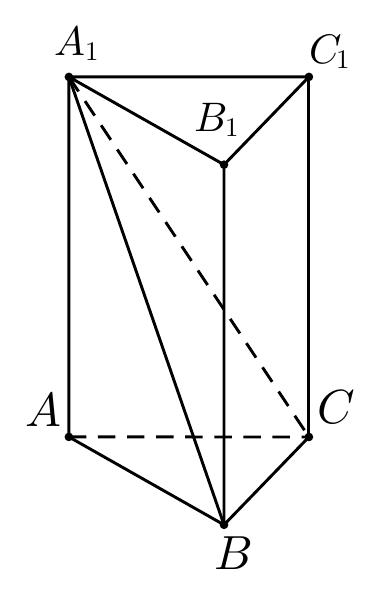
\begin{tikzpicture}[x=1mm,y=1mm,line width=0.370mm,line join=bevel,
  every node/.style={inner sep=0pt,outer sep=0pt}]
  % line join=bevel：源图角部无 miter 尖刺（A1 处两线交角 29.5°，miter 会长出 1.45mm，源图实测无）
  \path[use as bounding box] (0,0) rectangle (41.100,68.936);  % 源画布 691×1159px
  % ---- 顶点：10 条边逐线亚像素拟合后取交点（残差 <0.16px）；注释为源图像素坐标 ----
  \coordinate (A1) at ( 5.235,62.684);  % px( 88.008, 105.125)
  \coordinate (C1) at (35.717,62.684);  % px(600.498, 105.117)
  \coordinate (B1) at (24.936,51.534);  % px(419.239, 292.585)
  \coordinate (A)  at ( 5.234,16.961);  % px( 87.997, 873.843)
  \coordinate (C)  at (35.717,16.952);  % px(600.495, 873.999)
  \coordinate (B)  at (24.935, 5.798);  % px(419.225,1061.522)
  % ---- 线网：上底三边实线；三条侧棱实线；下底 AB、BC 实线、AC 虚线（被遮棱）；A1B 实线辅助线；CA1 虚线辅助线
  \draw (A1) -- (C1) -- (B1) -- cycle;
  \draw (A1) -- (A);
  \draw (B1) -- (B);
  \draw (C1) -- (C);
  \draw (A) -- (B) -- (C);
  \draw[dash pattern=on 2.214mm off 1.480mm] (A) -- (C);
  \draw (A1) -- (B);
  \draw[dash pattern=on 2.214mm off 1.480mm] (A1) -- (C);
  % ---- 六顶点实心点（半径 0.548mm＝源墨 0.531mm 扣口径校正）----
  \foreach \p in {A1,C1,B1,A,C,B} \fill (\p) circle[radius=0.548mm];
  % ---- 标签：anchor=base（y＝源图基线；x＝主体字墨心，均按源图墨 bbox 标定，偏差 <0.06mm）----
  \node[anchor=base,font=\fontsize{14.90pt}{17pt}\selectfont] at ( 6.226,65.363) {\qlabs{A}{1}{-0.117mm}}; % 源 px 基线 y=59 ,  墨心 x=87.0
  \node[anchor=base,font=\fontsize{14.90pt}{17pt}\selectfont] at (38.333,64.350) {\qlabs{C}{1}{-0.308mm}}; % 源 px 基线 y=77 ,  墨心 x=634.5
  \node[anchor=base,font=\fontsize{14.90pt}{17pt}\selectfont] at (24.037,55.768) {\qlabs{B}{1}{-0.096mm}}; % 源 px 基线 y=221,  墨心 x=389.0
  \node[anchor=base,font=\fontsize{17.30pt}{20pt}\selectfont] at ( 1.979,18.325) {\qlab{A}};                % 源 px 基线 y=850,  墨心 x=28.0
  \node[anchor=base,font=\fontsize{17.30pt}{20pt}\selectfont] at (38.991,18.712) {\qlab{C}};                % 源 px 基线 y=844,  墨心 x=657.0
  \node[anchor=base,font=\fontsize{17.30pt}{20pt}\selectfont] at (26.082, 0.063) {\qlab{B}};                % 源 px 基线 y=1157, 墨心 x=436.5
\end{tikzpicture}
% ==================== 片段止 ====================
\end{document}
